\documentclass[11pt
  , a4paper
  , article
  , oneside
  %  , twoside
  , showtrims
 % , draft
]{memoir}

\usepackage{essdocs}
\usepackage[numbers]{natbib}
\usepackage[autostyle]{csquotes}

%% \usepackage{epstopdf}
%% \usepackage[pdf]{pstricks}
%% \usepackage{graphicx}

\setsecnumdepth{subsection}

\begin{document}
%\frontmatter
%% ESS Document Description
%%
\essdocdesc{Engineering Manual}

%% ESS Document Number
%%
\essdocnum{ESS-XXXXXXXX}

%% Date
%%
\date{\today}

%% ESS Document Revision Number
%%
\essdocrev{0.1}

%% ESS Document State
%%
\essdocstate{Early Draft}

%% ESS Document Classification
%%
\essdocclass{ESS Use Only}

%% Document Title
%%
\title{ICS Engineering Manual}
\subtitle{for $\mu$TCA backplane clock distribution}
%% Document Author(s), if more than one author,
%% use \newline instead of \\ or \linebreak in order to seperate them
\author{Javier Cereijo Garcia \newline Simone Farina \newline Jeong Han Lee}

%% Document Reviewer(s) if more than one reviewer,
%% use \newline instead of \\ or \linebreak in order to seperate them
%\reviewer{Timo Korhonen (Chief Engineer) \newline Timo Korhonen (Chief Engineer)}
\reviewer{TBD}
%% Document Owner(s) if more than one owner,
%% use \newline instead of \\ or \linebreak in order to seperate them
\owner{ICS}

%% Document Approver(s) if more than one approver,
%% use \newline instead of \\ or \linebreak in order to seperate them
\approver{ICS}

\showtrimson

\esstitle
\newpage
\tableofcontents
\newpage

%\mainmatter


%%% Actual Document Start at below
\chapter{Overview}
At European Spallation Source (ESS), Integrated Control System (ICS) uses the Micro Research Finland (MRF) Timing System{\footnote{\url{http://www.mrf.fi/}}} as its timing system of the ESS site. The consistent and up-to-date engineering manual is essential for the ESS Timing system.

\section{Scope}
\begin{itemize}
\item This document explains how to configure a $\mu$TCA system to send the event clock from a MTCA-EVR-300(U) to an AMC using the backplane.
\item This document provides the configuration for the MCH and EVR, and guidelines for best practices on the use of the backplane clocks in the AMCs.
\end{itemize}
\textbf{Note that this is a very early draft document and should be updated as development progresses.}

\section{Target Audience}
This document is targeted to ICS engineers and technical stakeholders of the ESS timing system. It is assumed that the target audience has a technical background in the MRF Timing System, the EPICS development, and a Linux environment.


\chapter{System Description}
MRF Technical Reference \citep[see][p45]{MRFEVENTSYSTEMDC} explained Event Receivers and wrote :
\blockquote{\textit{Event Receivers decode timing events and signals from an optical event stream transmitted by an Event Generator. Events and signals are received at predefined rate the event clock that is usually divided down from an accelerators main RF reference. The event receivers lock to the phase event clock of the Event Generator and are thus phase locked to the RF reference. Event Receivers convert event codes transmitted by an Event Generator to hardware outputs. They can also generate software interrupts and store the event codes with globally distributed timestamps into FIFO memory to be read by a CPU.}}

ICS uses and will use the following different types of EVR :
\begin{itemize}
\item MTCA-EVR-300(U)
\item PCIe-EVR-300DC
\end{itemize}

One of the appealings of the MTCA-EVR-300(U) is its capability to send the event clock which is derived from and phase-locked to the main RF frequency to the AMCs via the backplane. For this the system should be configured in the approppriate way described in this document.

\section{MTCA.4 Standard}
The microTCA standard, sometimes reffered to as uTCA or MTCA is short for Micro Telecomunications Computing Architecture. The bare bone components needed in every MTCA.4 system are a crate/chassis that includes a backplane and cooling units (CUs), a power supply and an MCH (MTCA Carrier Hub). The crate can have up to four slots for power modules (PMs), up to two for MCHs and up to 12 AMC (Advance Mezzannine Card) slots. The crate itself is quite passive - in order to be able to use the the system at least one MCH has to be present in the system.

\subsection{MCH}
The MCH is inserted into a dedicated slot in the crate and manages the system. It takes care of routing connections between the system components and monitors the overall system status. It is also able to protect the system in case anything goes wrong.

Most of the configuration to send the event clock to an AMC is done in the MCH, since it's in charge of routing the connections over the $\mu$TCA backplane, including the clock lines.


\section{MTCA-EVR-300(U)}
Figure~\ref{fig:mtca-evr300} shows the rough physical dimensions $181\times 148~\mathrm{mm}{}^2$ of the MTCA-EVR-300 card.

\begin{figure}[!htb]
  \centering
  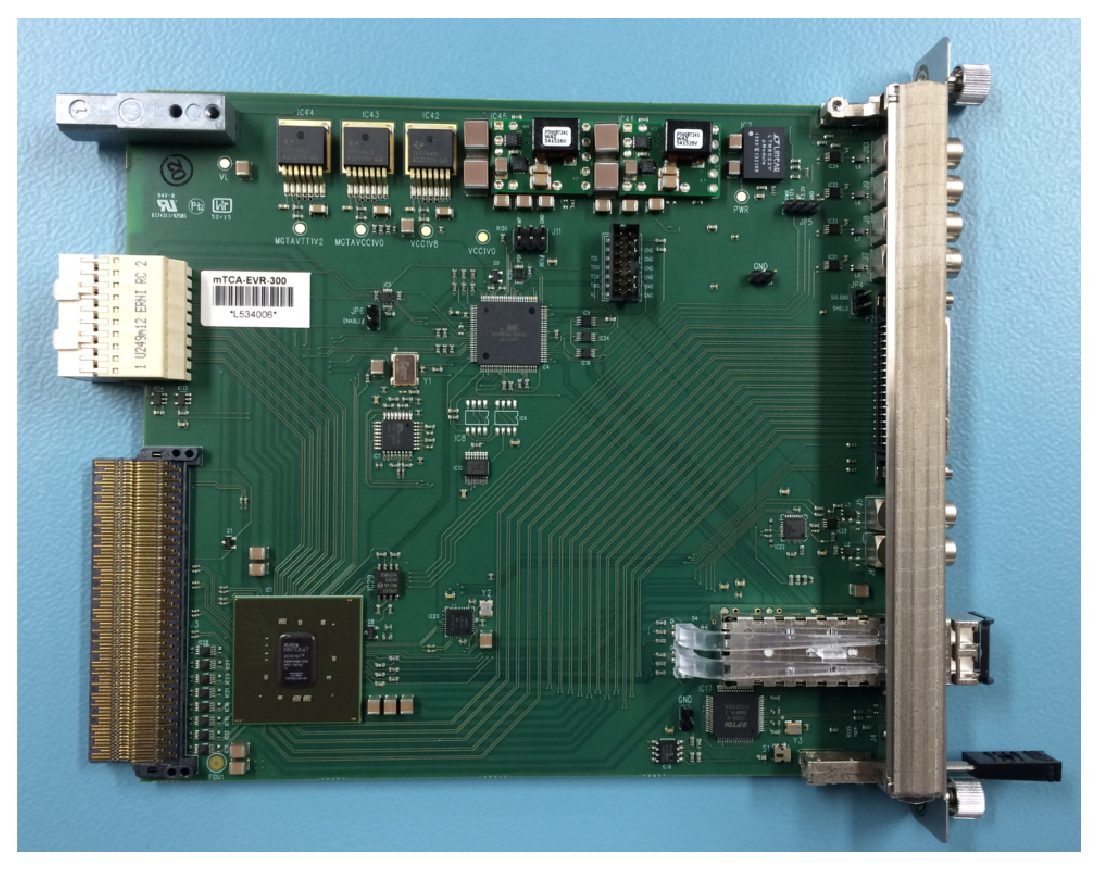
\includegraphics[width=0.99\textwidth]{./pictures/mtca_evr_300.eps}
  \caption{
    MRF MTCA-EVR-300 board.
  }
  \label{fig:mtca-evr300}
\end{figure}

The MTCA-EVR-300 has a SFP transceiver as an input from EVG and several outputs: 4 front panel outputs, 16 front universal outputs (through the IFB-300 extension board), 8 backplane trigger lines and 2 backplane clock lines. The 16 front universal outputs are implemented through a micro-SCSI type connector for an interface board IFB-300, which has eight Universal I/O slots. The MTCA-EVR-300U is identical but replaces the micro-SCSI connector for two Universal I/O slots.

\clearpage

\chapter{System Environment}
Before describing the engineering procedure for sending the event clock through the backplane, it is mandatory to have proper system environment that consists of specific hardware and software lists. Here we will show the hardware and software lists, their block diagrams, and their setup in the ICS lab at ESS. The information shown in this chapter is used in the ICS Lab at ESS.


\section{Hardware}
Table~\ref{table:hwlist} shows the hardware list and its environment. Here, \texttt{TAG} is used as the prefix of the ICS internal inventory system in order to track it down.
\begin{table}[!hb]
  \centering
  \begin{tabular}{l|l|l}
    \toprule
    Hardware                        & Info                                               & Serial Number \\\midrule
    MRF MTCA-EVR-300U               & \texttt{ICS TAG-521}                               & N012034       \\\midrule
    NAT-MCH-PHYS                    & \texttt{ICS TAG-747}                               & 113521-0786    \\\midrule
    Concurrent Technologies AMC CPU & \texttt{ICS TAG-726}                               & M29597/006     \\\midrule
    Schroff MTCA crate 12 slots, 9U    & \texttt{ICS TAG-723}                               & 11850026436032091321700490AC      \\\midrule
    Wiener power supply unit 1000W  & \texttt{ICS TAG-803}                               & 0985052       \\\midrule
    Ethernet cables                 &                                                    &               \\\bottomrule
  \end{tabular}
  \caption[]{Hardware List and Its Environment.}
  \label{table:hwlist}
\end{table}


Figure~\ref{fig:mtca-system} shows the MTCA-EVR-300U setup in the lab. From left to right, the power supply, MCH, CPU and MTCA-EVR-300U.
\begin{figure}[!b]
  \centering
  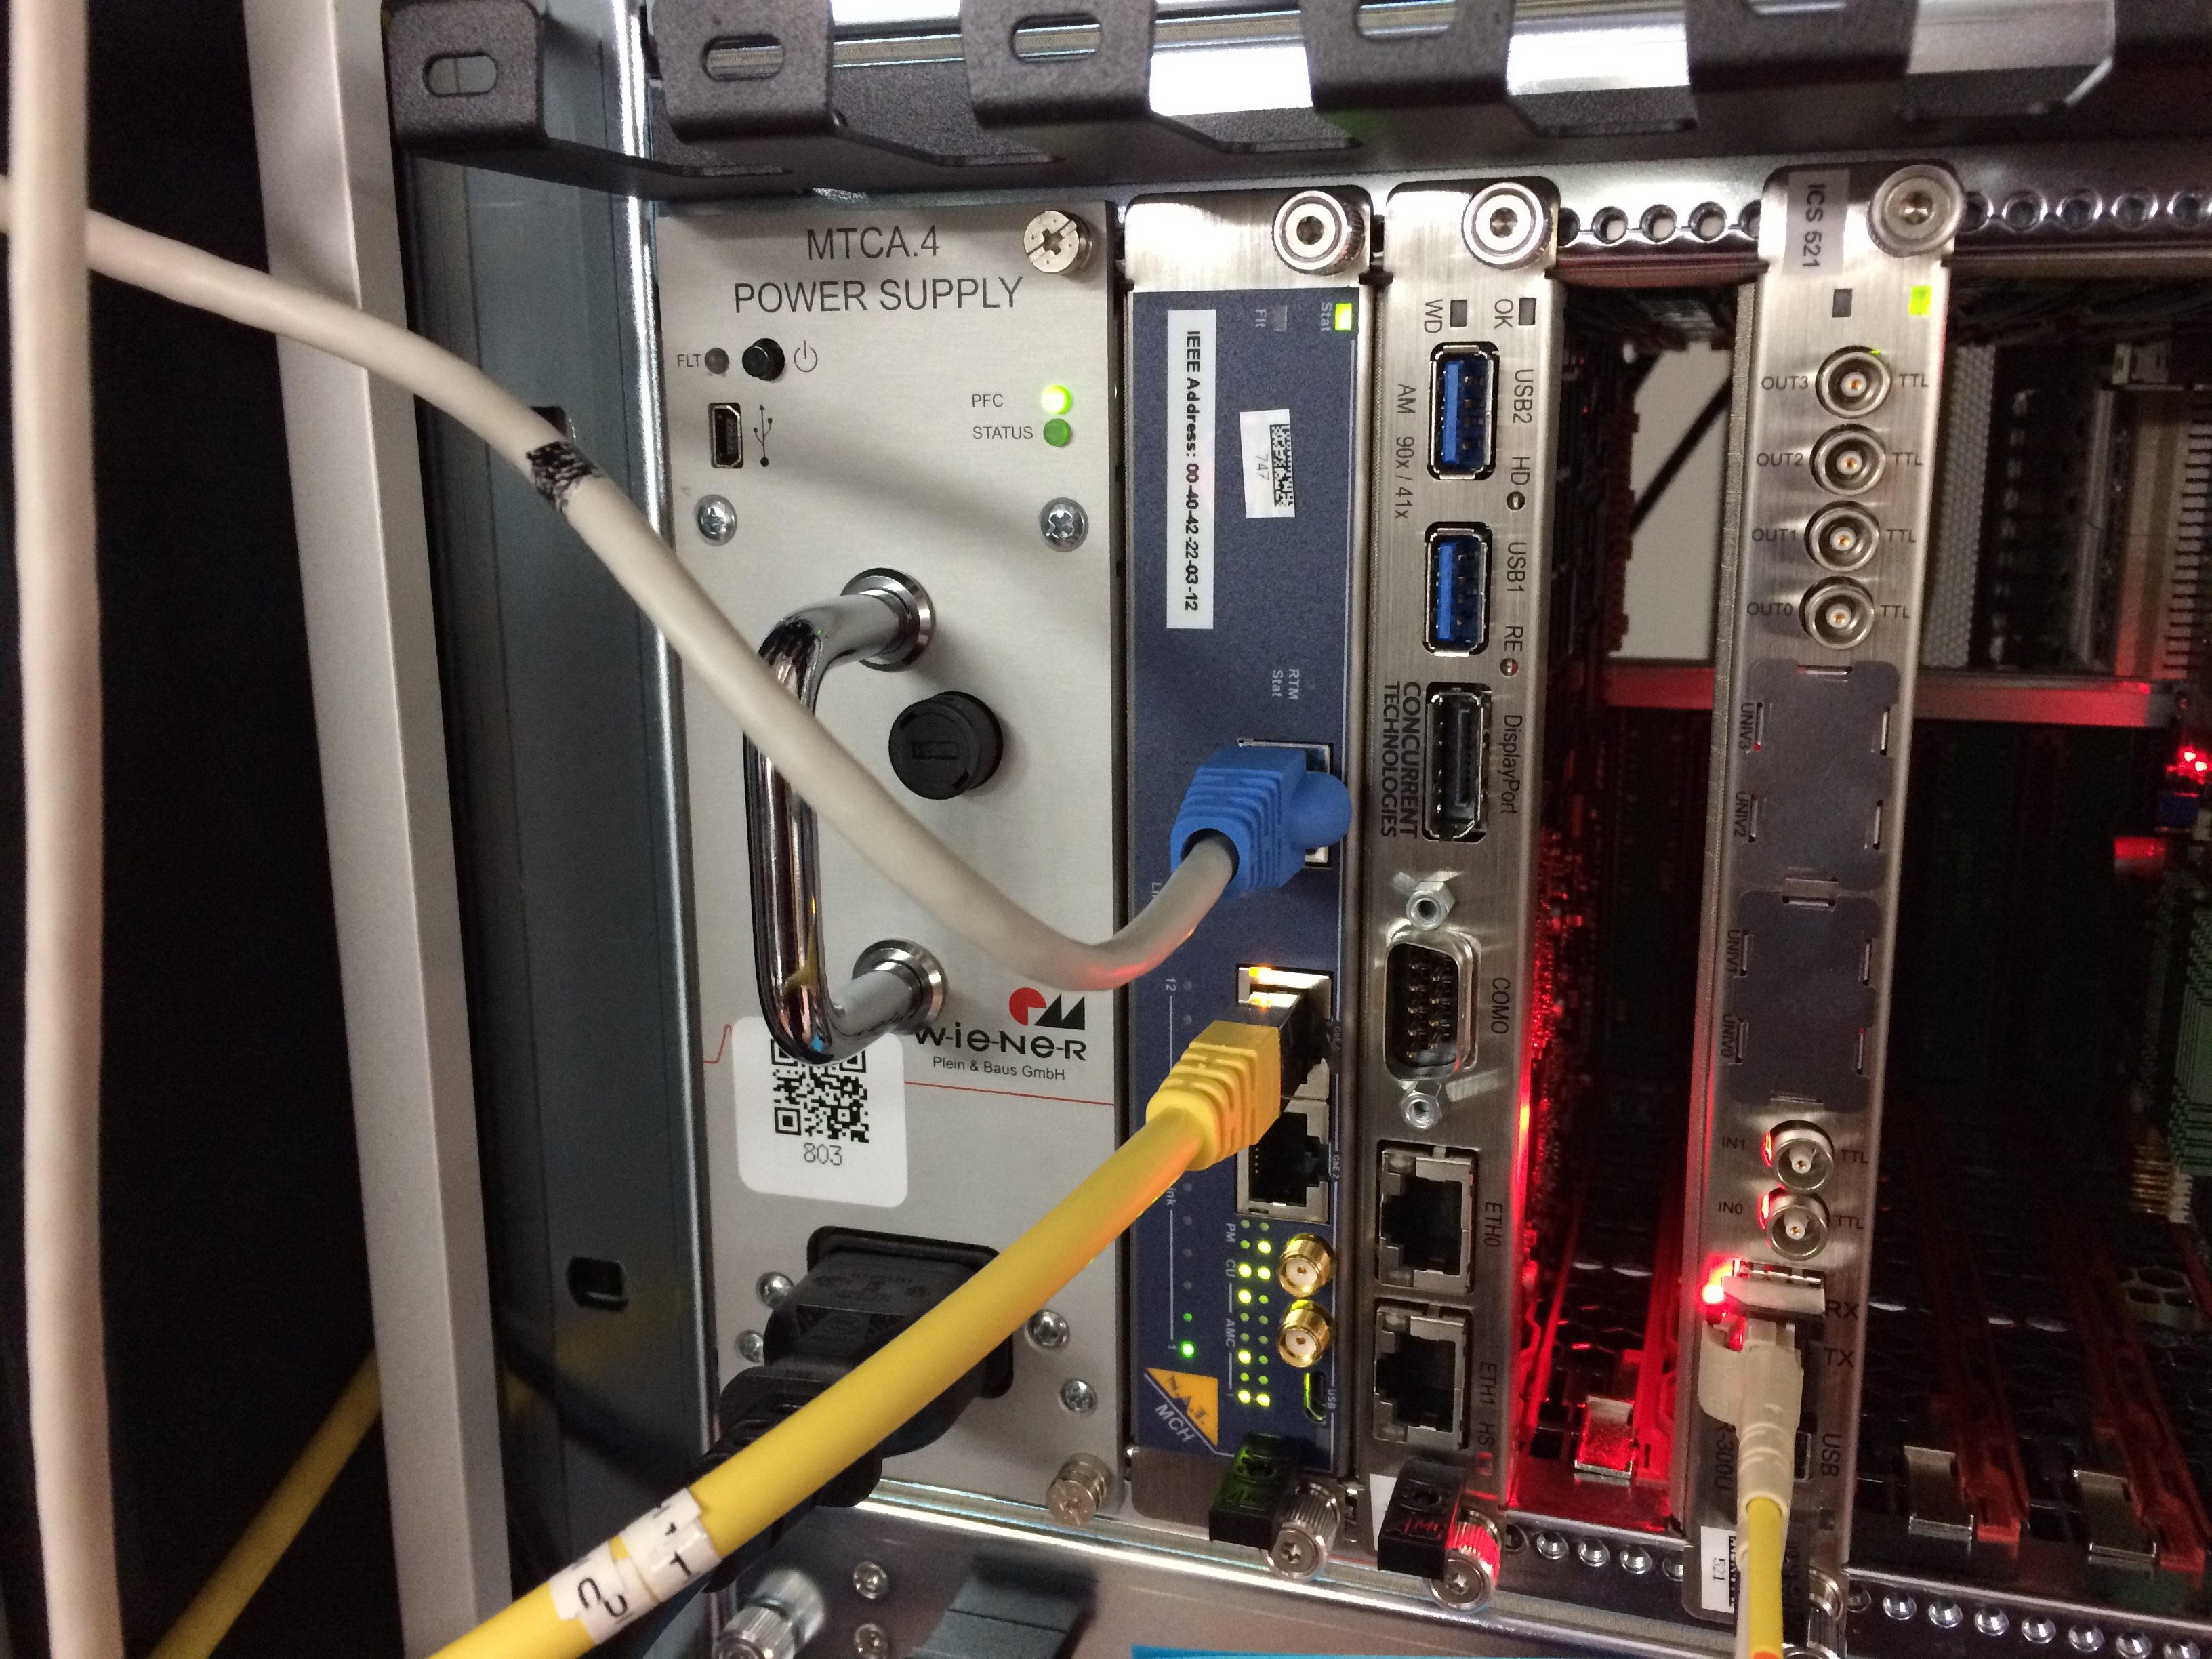
\includegraphics[width=0.8\textwidth]{./pictures/mtca_system.jpg}
  \caption{Hardware Setup in the ICS lab.}
  \label{fig:mtca-system}
\end{figure}


\clearpage
\section{Software}
Table~\ref{table:swlist} shows the Software list and its environment.
\begin{table}[!htb]
  \centering
  \begin{tabular}{l|l}
    \toprule
    Item               & Version Info.                                                       \\\midrule
    CentOS Linux       & \texttt{7.4.1708}                                                   \\\midrule
    Kernel             & \texttt{3.10.0-693.17.1.el7.x86\_64}                                 \\\midrule
    mrf kernel module  & version : \texttt{1} / srcversion \texttt{A998B22F1425D7388F5F7A7}  \\\midrule
    EPICS Base         & \texttt{3.15.5}                                                     \\\midrule
    mrfioc2            & Community or E3 ver. \texttt{2.2.0}                                     \\\midrule
    devLib2            & Community or E3 ver. \texttt{2.9.0}                                      \\\bottomrule
  \end{tabular}
  \caption[]{Software and its version information.}
  \label{table:swlist}
\end{table}


\clearpage
\chapter{Engineering Procedure}
This chapter explains how to configure the system to send the event clock via the backplane.

\section{MCH configuration}
To configure the MCH, it is necessary to access its web interface. You can read how to access it in \citep{NATMCHWEBINTERFACE}.

In the menu on the left, click in \texttt{Script Management} under \texttt{Maintenance}. The MCH will take a couple of seconds to prepare the configuration script, as shown in Figure~\ref{fig:configfile}.
\begin{figure}[!htb]
  \centering
  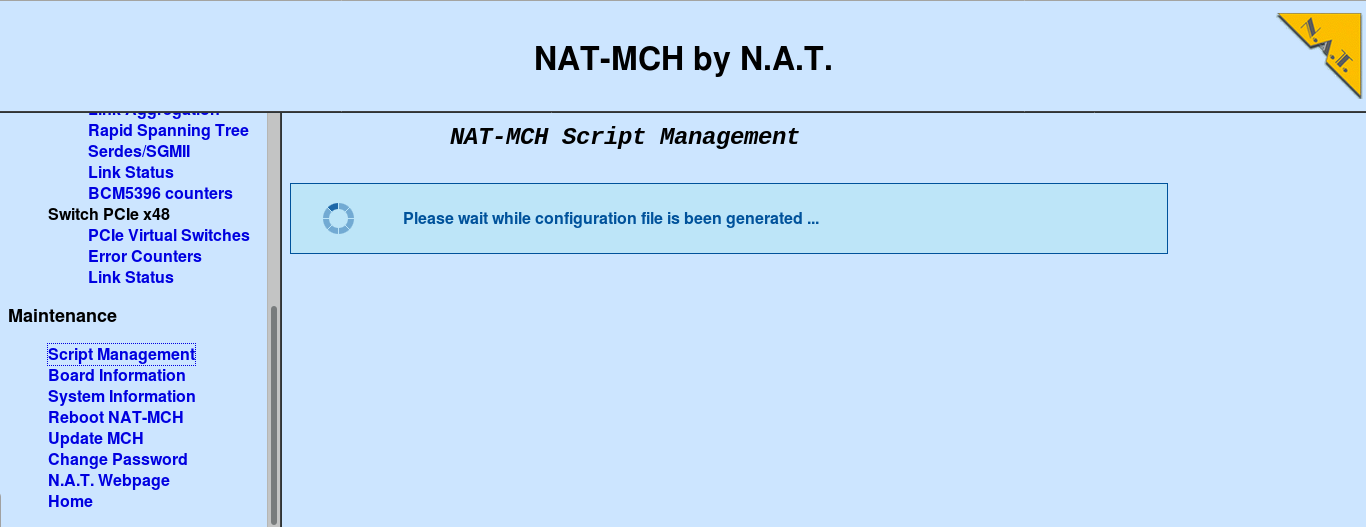
\includegraphics[width=0.8\textwidth]{./pictures/Configuration_file.png}
  \caption{Configuration script being generated.}
  \label{fig:configfile}
\end{figure}

Once the script is generated, the page will look like in Figure~\ref{fig:scriptmanagement}. The best way of configuring the MCH is to take the running configuration and modify it according to our needs. To do this click on \texttt{nat\_mch\_running\_cfg.txt} and download the file.

\begin{figure}[!htb]
  \centering
  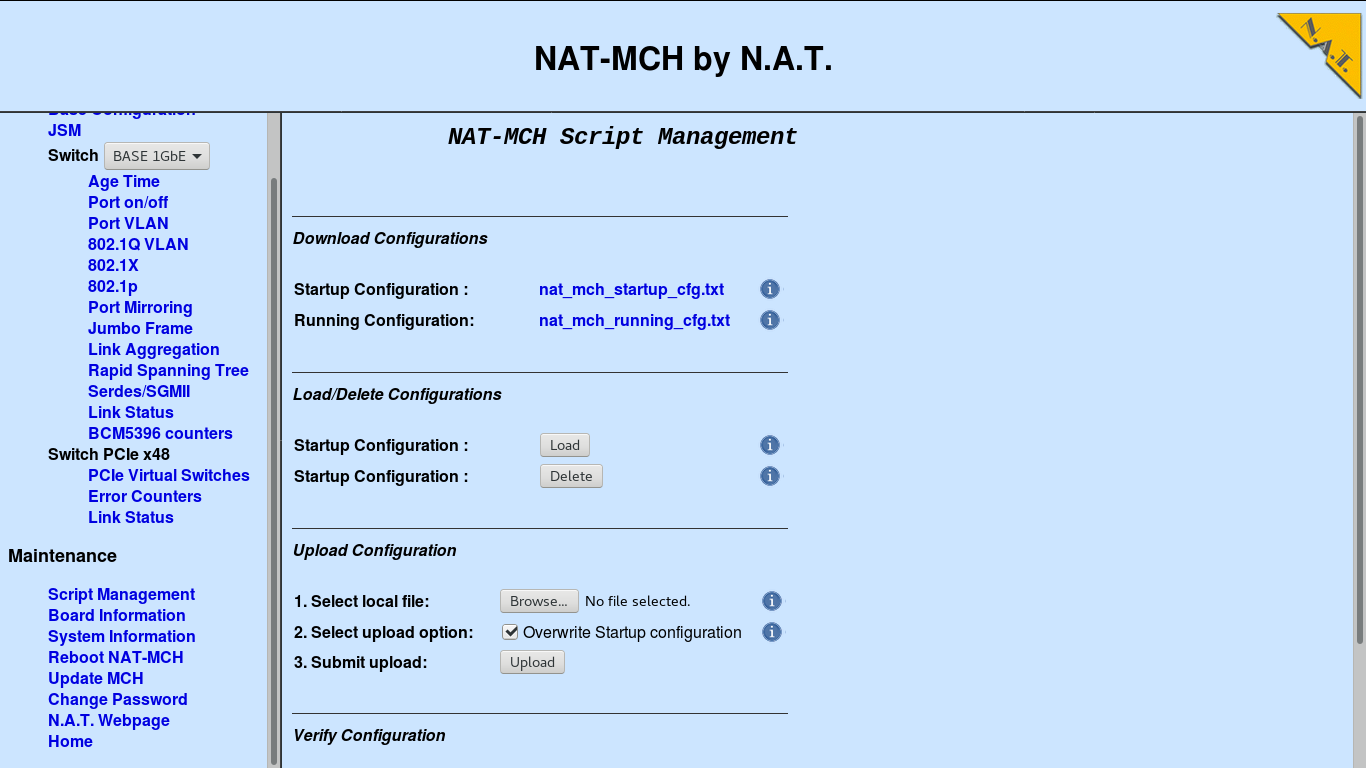
\includegraphics[width=0.8\textwidth]{./pictures/Script_management.png}
  \caption{Script management menu.}
  \label{fig:scriptmanagement}
\end{figure}

Open the file and look for the clock output configuration (\texttt{clk\_phys\_out}) section:
\begin{lstlisting}[style=termstyle]
#
# Item <<clk_phys_out>>: clock output configuration
#
# Syntax: clk_phys_out = dst, src
#
# NOTE: For optimal jitter performance unused inputs should be configured as
#       outputs driving a signal with minimum signal transitions!
#
# HCSL buffer detected
# - any source for CLK 3 output other then 0 will enable output of HCSL buffer
#
# Params: dst: destination clock identifier
#                1 -  CLK1 AMC  1
#                2 -  CLK1 AMC  2
#                3 -  CLK1 AMC  3
#                4 -  CLK1 AMC  4
#                5 -  CLK1 AMC  5
#                6 -  CLK1 AMC  6
#                7 -  CLK1 AMC  7
#                8 -  CLK1 AMC  8
#                9 -  CLK1 AMC  9
#               10 -  CLK1 AMC 10
#               11 -  CLK1 AMC 11
#               12 -  CLK1 AMC 12
#                          X
#                          X
#                          X
#                          X
#               17 -  CLK2 AMC  1
#               18 -  CLK2 AMC  2
#               19 -  CLK2 AMC  3
#               20 -  CLK2 AMC  4
#               21 -  CLK2 AMC  5
#               22 -  CLK2 AMC  6
#               23 -  CLK2 AMC  7
#               24 -  CLK2 AMC  8
#               25 -  CLK2 AMC  9
#               26 -  CLK2 AMC 10
#               27 -  CLK2 AMC 11
#               28 -  CLK2 AMC 12
#                          X
#                          X
#                          X
#                          X
#               33 -  CLK3 AMC  1
#               34 -  CLK3 AMC  2
#               35 -  CLK3 AMC  3
#               36 -  CLK3 AMC  4
#               37 -  CLK3 AMC  5
#               38 -  CLK3 AMC  6
#               39 -  CLK3 AMC  7
#               40 -  CLK3 AMC  8
#               41 -  CLK3 AMC  9
#               42 -  CLK3 AMC 10
#               43 -  CLK3 AMC 11
#               44 -  CLK3 AMC 12
#               48 -  EXT single ended 2 (OUTPUT SMA 1)
#               50 -  EXT single ended 4 (OUTPUT SMA 2)
#
# Params: src: source clock identifier
#                0 -  disabled
#                1 -  CLK1 AMC  1
#                2 -  CLK1 AMC  2
#                3 -  CLK1 AMC  3
#                4 -  CLK1 AMC  4
#                5 -  CLK1 AMC  5
#                6 -  CLK1 AMC  6
#                7 -  CLK1 AMC  7
#                8 -  CLK1 AMC  8
#                9 -  CLK1 AMC  9
#               10 -  CLK1 AMC 10
#               11 -  CLK1 AMC 11
#               12 -  CLK1 AMC 12
#                          X
#                          X
#                          X
#                          X
#               17 -  CLK2 AMC  1
#               18 -  CLK2 AMC  2
#               19 -  CLK2 AMC  3
#               20 -  CLK2 AMC  4
#               21 -  CLK2 AMC  5
#               22 -  CLK2 AMC  6
#               23 -  CLK2 AMC  7
#               24 -  CLK2 AMC  8
#               25 -  CLK2 AMC  9
#               26 -  CLK2 AMC 10
#               27 -  CLK2 AMC 11
#               28 -  CLK2 AMC 12
#               35 -  EXT single ended 1 (INPUT  SMA 1)
#               37 -  EXT single ended 3 (INPUT  SMA 2)
#               41 -  100MHz OSC (only with HCSL option)
#

clk_phys_out =  1,  0
clk_phys_out =  2,  0
clk_phys_out =  3,  0
clk_phys_out =  4,  0
clk_phys_out =  5,  0
clk_phys_out =  6,  0
clk_phys_out =  7,  0
clk_phys_out =  8,  0
clk_phys_out =  9,  0
clk_phys_out = 10,  0
clk_phys_out = 11,  0
clk_phys_out = 12,  0
clk_phys_out = 13,  0
clk_phys_out = 14,  0
clk_phys_out = 15,  0
clk_phys_out = 16,  0
clk_phys_out = 17,  0
clk_phys_out = 18,  0
clk_phys_out = 19,  0
clk_phys_out = 20,  0
clk_phys_out = 21,  0
clk_phys_out = 22,  0
clk_phys_out = 23,  0
clk_phys_out = 24,  0
clk_phys_out = 25,  0
clk_phys_out = 26,  0
clk_phys_out = 27,  0
clk_phys_out = 28,  0
clk_phys_out = 29,  0
clk_phys_out = 30,  0
clk_phys_out = 31,  0
clk_phys_out = 32,  0
clk_phys_out = 33,  0
clk_phys_out = 34,  0
clk_phys_out = 35,  0
clk_phys_out = 36,  0
clk_phys_out = 37,  0
clk_phys_out = 38,  0
clk_phys_out = 39,  0
clk_phys_out = 40,  0
clk_phys_out = 41,  0
clk_phys_out = 42,  0
clk_phys_out = 43,  0
clk_phys_out = 44,  0
clk_phys_out = 48,  0
clk_phys_out = 50,  0

\end{lstlisting}

This section tells the MCH how to configure the clock lines. Although it is not mandatory, the standard is to use line TCLKB/CLK2 to send the clock from the source (the EVR in our case) to the MCH, and line TCLKA/CLK1 to distribute that same clock to the rest of the AMCs, so doing it in this way is encouraged. First check what AMC slot the EVR is installed in (slot 3 for this example, as can be seen in Figure~\ref{fig:mtca-system}), and look what identifier code is related to that AMC slot for CLK2 in the MHC's configuration script \texttt{Params: src: source clock identifier} subsection of the \texttt{clock output configuration} section (\texttt{19 -  CLK2 AMC  3} in our example). Then in the same way find the identifier code of the AMC slot you want to send the event clock to in the \texttt{Params: dst: destination clock identifier} subsection (in our example AMC slots 1 to 12, except 3 where the EVR is installed).

Next do the same with \texttt{source clock identifier 100MHz OSC (only with HCSL option)} (41) and \texttt{destination clock identifier} CLK3 AMC 1 to 12 (33-44).

Finally for every destination identifier write a line with the following format:
\begin{lstlisting}[style=termstyle]
clk_phys_out =  destination_clock_identifier  source_clock_identifier
\end{lstlisting}
right at the end of the clock output configuration (\texttt{clk\_phys\_out}) section. \textbf{Note that there is a bug in some FW versions so the MCH will show an error when selecting the same identifier as source as destination, so that line will have to left at source 0 in that FW.}

In our example the section will look like this:
\begin{lstlisting}[style=termstyle]
#
# Item <<clk_phys_out>>: clock output configuration
#
# Syntax: clk_phys_out = dst, src
#
# NOTE: For optimal jitter performance unused inputs should be configured as
#       outputs driving a signal with minimum signal transitions!
#
# HCSL buffer detected
# - any source for CLK 3 output other then 0 will enable output of HCSL buffer
#
# Params: dst: destination clock identifier
#                1 -  CLK1 AMC  1
#                2 -  CLK1 AMC  2
#                3 -  CLK1 AMC  3
#                4 -  CLK1 AMC  4
#                5 -  CLK1 AMC  5
#                6 -  CLK1 AMC  6
#                7 -  CLK1 AMC  7
#                8 -  CLK1 AMC  8
#                9 -  CLK1 AMC  9
#               10 -  CLK1 AMC 10
#               11 -  CLK1 AMC 11
#               12 -  CLK1 AMC 12
#                          X
#                          X
#                          X
#                          X
#               17 -  CLK2 AMC  1
#               18 -  CLK2 AMC  2
#               19 -  CLK2 AMC  3
#               20 -  CLK2 AMC  4
#               21 -  CLK2 AMC  5
#               22 -  CLK2 AMC  6
#               23 -  CLK2 AMC  7
#               24 -  CLK2 AMC  8
#               25 -  CLK2 AMC  9
#               26 -  CLK2 AMC 10
#               27 -  CLK2 AMC 11
#               28 -  CLK2 AMC 12
#                          X
#                          X
#                          X
#                          X
#               33 -  CLK3 AMC  1
#               34 -  CLK3 AMC  2
#               35 -  CLK3 AMC  3
#               36 -  CLK3 AMC  4
#               37 -  CLK3 AMC  5
#               38 -  CLK3 AMC  6
#               39 -  CLK3 AMC  7
#               40 -  CLK3 AMC  8
#               41 -  CLK3 AMC  9
#               42 -  CLK3 AMC 10
#               43 -  CLK3 AMC 11
#               44 -  CLK3 AMC 12
#               48 -  EXT single ended 2 (OUTPUT SMA 1)
#               50 -  EXT single ended 4 (OUTPUT SMA 2)
#
# Params: src: source clock identifier
#                0 -  disabled
#                1 -  CLK1 AMC  1
#                2 -  CLK1 AMC  2
#                3 -  CLK1 AMC  3
#                4 -  CLK1 AMC  4
#                5 -  CLK1 AMC  5
#                6 -  CLK1 AMC  6
#                7 -  CLK1 AMC  7
#                8 -  CLK1 AMC  8
#                9 -  CLK1 AMC  9
#               10 -  CLK1 AMC 10
#               11 -  CLK1 AMC 11
#               12 -  CLK1 AMC 12
#                          X
#                          X
#                          X
#                          X
#               17 -  CLK2 AMC  1
#               18 -  CLK2 AMC  2
#               19 -  CLK2 AMC  3
#               20 -  CLK2 AMC  4
#               21 -  CLK2 AMC  5
#               22 -  CLK2 AMC  6
#               23 -  CLK2 AMC  7
#               24 -  CLK2 AMC  8
#               25 -  CLK2 AMC  9
#               26 -  CLK2 AMC 10
#               27 -  CLK2 AMC 11
#               28 -  CLK2 AMC 12
#               35 -  EXT single ended 1 (INPUT  SMA 1)
#               37 -  EXT single ended 3 (INPUT  SMA 2)
#               41 -  100MHz OSC (only with HCSL option)
#

clk_phys_out =  1,  19
clk_phys_out =  2,  19
clk_phys_out =  3,  0
clk_phys_out =  4,  19
clk_phys_out =  5,  19
clk_phys_out =  6,  19
clk_phys_out =  7,  19
clk_phys_out =  8,  19
clk_phys_out =  9,  19
clk_phys_out = 10,  19
clk_phys_out = 11,  19
clk_phys_out = 12,  19
clk_phys_out = 13,  0
clk_phys_out = 14,  0
clk_phys_out = 15,  0
clk_phys_out = 16,  0
clk_phys_out = 17,  0
clk_phys_out = 18,  0
clk_phys_out = 19,  0
clk_phys_out = 20,  0
clk_phys_out = 21,  0
clk_phys_out = 22,  0
clk_phys_out = 23,  0
clk_phys_out = 24,  0
clk_phys_out = 25,  0
clk_phys_out = 26,  0
clk_phys_out = 27,  0
clk_phys_out = 28,  0
clk_phys_out = 29,  0
clk_phys_out = 30,  0
clk_phys_out = 31,  0
clk_phys_out = 32,  0
clk_phys_out = 33,  41
clk_phys_out = 34,  41
clk_phys_out = 35,  41
clk_phys_out = 36,  41
clk_phys_out = 37,  41
clk_phys_out = 38,  41
clk_phys_out = 39,  41
clk_phys_out = 40,  41
clk_phys_out = 41,  0
clk_phys_out = 42,  41
clk_phys_out = 43,  41
clk_phys_out = 44,  41
clk_phys_out = 48,  0
clk_phys_out = 50,  0

\end{lstlisting}

The script has to be uploaded to the MCH's web interface. In the \texttt{Script Management} menu, under the \texttt{Upload Configuration} section, click on \texttt{Select local file: Browse...} and select the configuration file, check (if not already) the \texttt{Select upload option: Overwrite Startup configuration}, and click \texttt{Submit upload:Upload}.

Finally go to the \texttt{Base Configuration} on the left menu, and in the \texttt{Clock module parameter} section select \texttt{load from FLASH}. Go all the way down and click on \texttt{Save}.

After these steps the MCH should be properly configured. If there is some error try power cycling the MCH.


\section{mTCA-EVR-300(U) configuration}
For a general introduction to the EVR, please check \citep{EVRMANUAL}. \textbf{Note that, as shown in Table~\ref{table:swlist}, mrfioc2 community or E3 version 2.2.0 is needed.}

Start an EVR IOC as usual and set the following records as shown; this assumes TCLKB/CLK2 is used to send the clock from the EVR to the MCH as previously explained:
\begin{lstlisting}[style=termstyle]
# Set TCLKB to low, enable it and power it up
dbpf $(IOC)-$(DEV1):OutTCLKB-Src-SP 63
dbpf $(IOC)-$(DEV1):OutTCLKB-Ena-Sel 1
dbpf $(IOC)-$(DEV1):OutTCLKB-Pwr-Sel 1

# TCLKB is 40-bit pattern, set the starting 20 bits to 1 (and the rest to 0 - default)
dbpf $(IOC)-$(DEV1):OutTCLKB-Pat-Low00_15-SP.BF 1
dbpf $(IOC)-$(DEV1):OutTCLKB-Pat-Low00_15-SP.BE 1
dbpf $(IOC)-$(DEV1):OutTCLKB-Pat-Low00_15-SP.BD 1
dbpf $(IOC)-$(DEV1):OutTCLKB-Pat-Low00_15-SP.BC 1
dbpf $(IOC)-$(DEV1):OutTCLKB-Pat-Low00_15-SP.BB 1
dbpf $(IOC)-$(DEV1):OutTCLKB-Pat-Low00_15-SP.BA 1
dbpf $(IOC)-$(DEV1):OutTCLKB-Pat-Low00_15-SP.B9 1
dbpf $(IOC)-$(DEV1):OutTCLKB-Pat-Low00_15-SP.B8 1
dbpf $(IOC)-$(DEV1):OutTCLKB-Pat-Low00_15-SP.B7 1
dbpf $(IOC)-$(DEV1):OutTCLKB-Pat-Low00_15-SP.B6 1
dbpf $(IOC)-$(DEV1):OutTCLKB-Pat-Low00_15-SP.B5 1
dbpf $(IOC)-$(DEV1):OutTCLKB-Pat-Low00_15-SP.B4 1
dbpf $(IOC)-$(DEV1):OutTCLKB-Pat-Low00_15-SP.B3 1
dbpf $(IOC)-$(DEV1):OutTCLKB-Pat-Low00_15-SP.B2 1
dbpf $(IOC)-$(DEV1):OutTCLKB-Pat-Low00_15-SP.B1 1
dbpf $(IOC)-$(DEV1):OutTCLKB-Pat-Low00_15-SP.B0 1
dbpf $(IOC)-$(DEV1):OutTCLKB-Pat-Low16_31-SP.BF 1
dbpf $(IOC)-$(DEV1):OutTCLKB-Pat-Low16_31-SP.BE 1
dbpf $(IOC)-$(DEV1):OutTCLKB-Pat-Low16_31-SP.BD 1
dbpf $(IOC)-$(DEV1):OutTCLKB-Pat-Low16_31-SP.BC 1
\end{lstlisting}



\section{AMC configuration}
If everything is set as explained before, TCLKB/CLK2 will deliver the event clock from the EVR to the MCH, and the MCH will then distribute the clock to the AMCs using TCLKA/CLK1. Configure the AMC so that it is expecting the clock in this line.


\clearpage

\backmatter
%\bibliographystyle{unsrt}
%\bibliographystyle{plainnat}
%\bibliographystyle{abbrvnat}
\bibliographystyle{unsrtnat}
%\bibliographystyle{chicago}
%\bibliography{./ess_refs}
\bibliography{mtca_backplane_clocks}

\end{document}
